\section{Method}
The architecture of of our project is shown as follows. Given a software project in Java, we select the most important files as an input for extracting parsed trees in the form of ASTs. Next, we convert from tree structure of AST to sequences of AST node types. From this sequence, we transform them to a vector represented features of source code.Finally, the ML classification models will predict the range of stars for project, while the ML regression model gives developer information about actual number of stars he/she can get in the next 2 years.

\begin{figure}
        \center{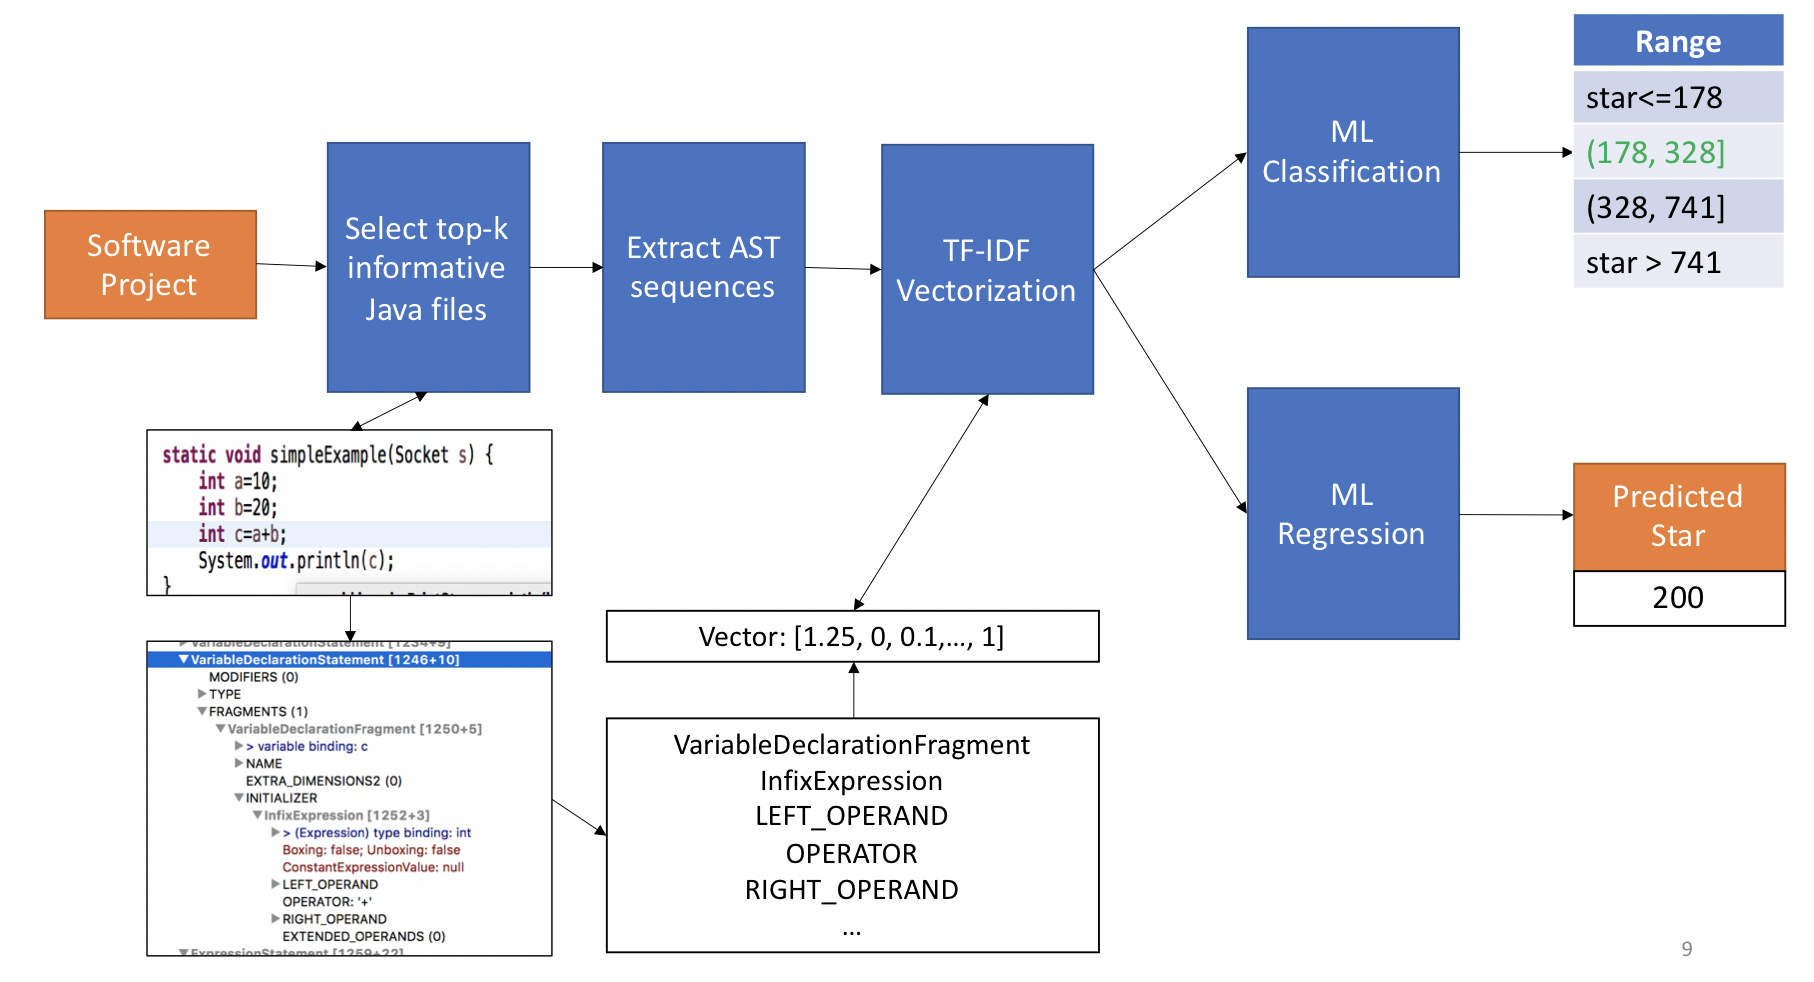
\includegraphics[width=\linewidth]
        {images/code_architecture.png}}
        \caption{Code based Github Projects Star Prediction Overview}
        \label{fig:mapping_expression} 
\end{figure}
\subsection{Select Top-k Java Files}
The ideal solution for representing the code is to extract information about all textual files inside a Java Github project. However, this approach can be very expensive since the number of files for each industrial project can be more than 10000. More over, by experiment, we see that TF-IDF can only be scalable with small set of documents with less than 100. So, our design choice select top 50 most important files as source code. The criteria for selecting files is choosing the files with most number of \texttt{import} statements in the project. We assume that a file used multiple APIs means it is developed to solve important tasks.
\subsection{Extract AST Sequences}
Big code can contain large vocabulary \cite{015}. This fact can also bring the vectorization ended with very sparse matrix of vocabularity for each software project, which decreases the performance of TF-IDF drastically. To overcome this problem, we extract the sequence of non-terminal AST nodes instead of actual tokens. In example shows in Figure \ref{fig:mapping_expression}, we extract the AST nodes related to expression and variable declaration. The vocabulary for single word is limited to over 82 types of ASTs defined in \cite{007}.
\subsection{Range of stars for Classification}
\subsection{Optimization for TF-IDF Vectorization}
\subsection{Hyper Parameter Tuning for Support Vector Machine Classification}
\subsection{Hyper Parameter Tuning for XG Boost Regression}


